% ============================================================================
\section{Normalization}
% ============================================================================

\begin{frame}{Transformer Block}
  \begin{itemize}
    \item[\textcolor{red}{$\blacktriangleright$}] \textbf{Multi-head Attention}
    \item[\textcolor{red}{$\blacktriangleright$}] \textbf{Add \& Norm}
    \item[\textcolor{red}{$\blacktriangleright$}] \textbf{Feed-forward Layer}
    \item[\textcolor{red}{$\blacktriangleright$}] \textbf{Add \& Norm}
  \end{itemize}
  \vspace{1em}
  \textcolor{blue}{\textbf{Note}}\\
  Residual connections and layer normalization are crucial for effective training.
\end{frame}

\begin{frame}{Transformer Block}
  \centering
  
\includegraphics[width=\paperwidth,height=0.95\paperheight,keepaspectratio]{assets/Lecture-6_Introduction_to_Transformers/pdf_page_054.png}
\end{frame}



\begin{frame}{Pre-LayerNorm vs.\ Post-LayerNorm}
  \small
  \begin{table}[ht]
    \centering
    \begin{tabular}{lcc}
      \toprule
      \textbf{Feature} & \textbf{Pre-LN} & \textbf{Post-LN} \\
      \midrule
      Stability & \checkmark\,More stable & \ding{55}\,Less stable \\
      Gradient flow & \checkmark\,Better & \ding{55}\,Can explode/vanish \\
      Used in & GPT-3, T5 & Original Transformer \\
      \bottomrule
    \end{tabular}
    \caption*{\footnotesize\textbf{Table 1:} Comparison of Pre-LayerNorm and Post-LayerNorm Architectures}
  \end{table}

  \vspace{1em}

  \textbf{Pre-LN:} LayerNorm applied \textbf{before} sublayers

  \textbf{Post-LN:} LayerNorm applied \textbf{after} sublayers
\end{frame}

\begin{frame}{Pre-LayerNorm vs.\ Post-LayerNorm}
  \centering
  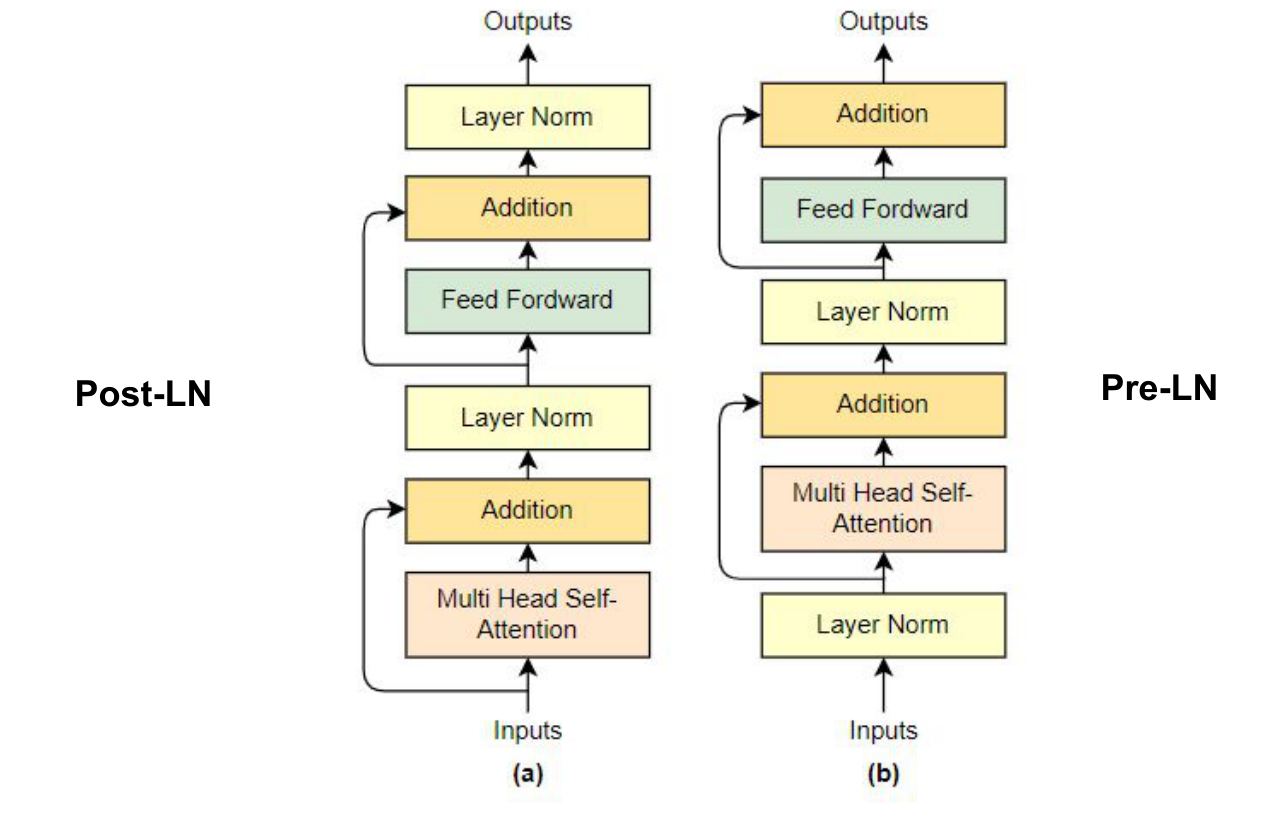
\includegraphics[width=0.8\paperwidth,height=0.8\paperheight,keepaspectratio]{assets/Lecture-6_Introduction_to_Transformers/pdf_page_084.png}
\end{frame}

\begin{frame}{Pre-LayerNorm vs.\ Post-LayerNorm}
  \centering
  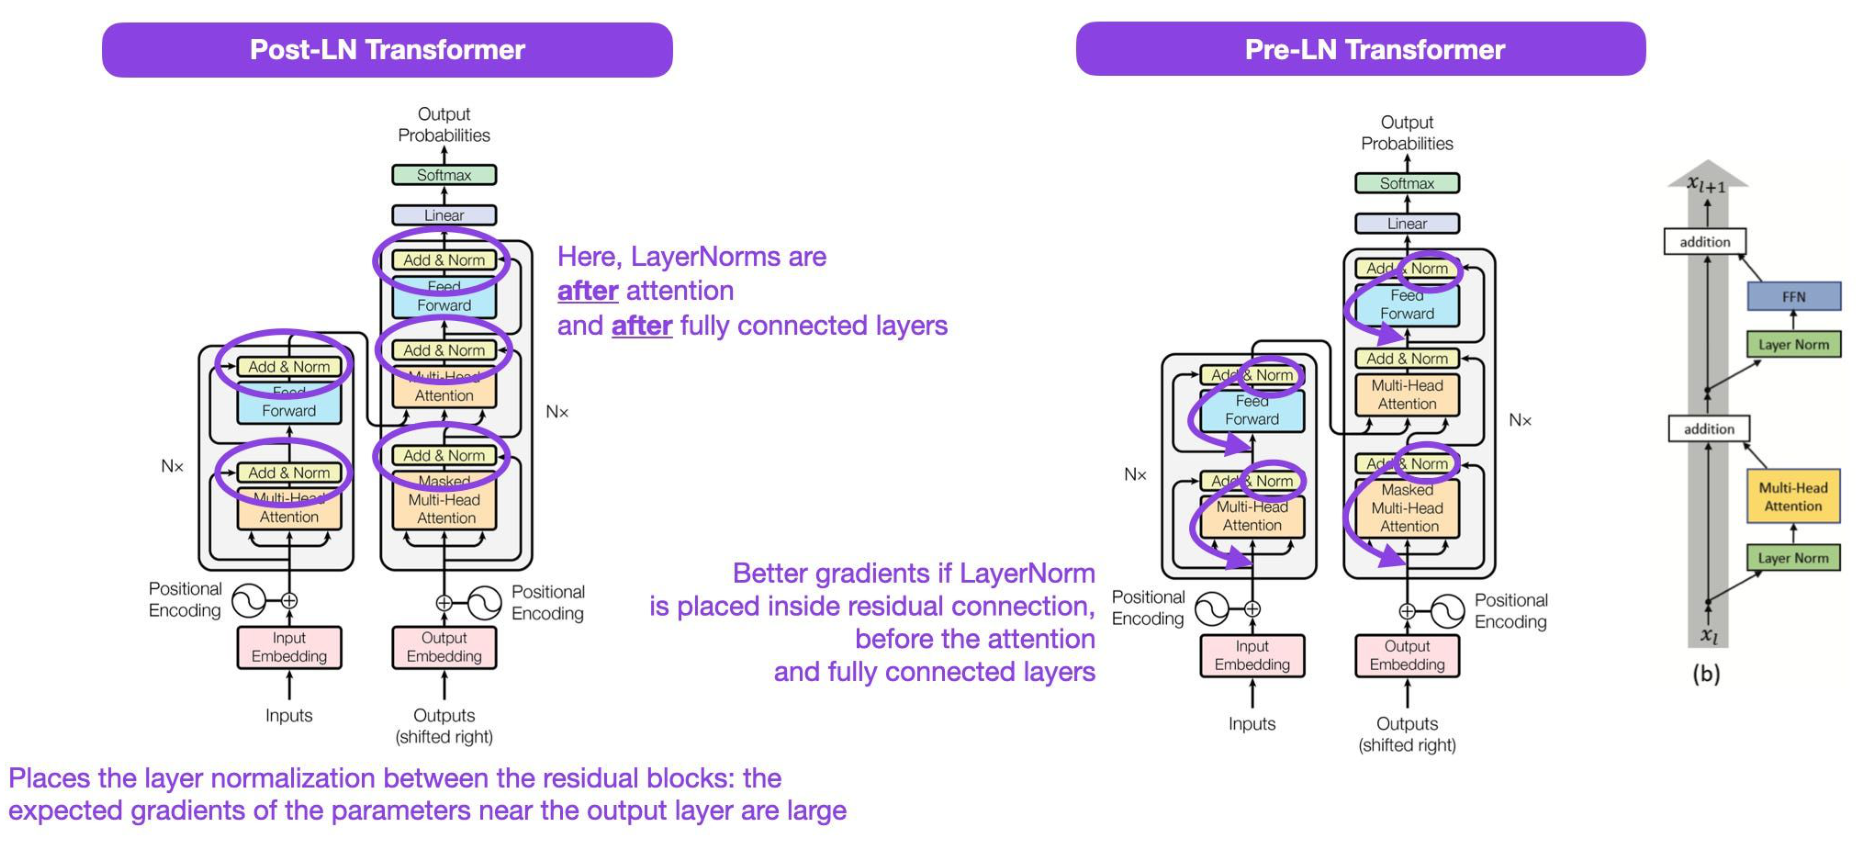
\includegraphics[width=0.9\paperwidth,height=0.9\paperheight,keepaspectratio]{assets/Lecture-6_Introduction_to_Transformers/pdf_page_085.png}
\end{frame} 

\begin{frame}{Layer Normalization vs RMSNorm}
  \small
  \textbf{LayerNorm:} Normalizes across the feature dimension by subtracting the mean and dividing by the standard deviation.

  \vspace{0.5em}
  \textbf{RMSNorm:} Does not shift the mean; scales by the root mean square (RMS) of the features.

  \vspace{1em}
  \begin{itemize}
      \item[$\blacktriangleright$] Simpler
      \item[$\blacktriangleright$] Faster
      \item[$\blacktriangleright$] Slightly better in large-scale settings.
  \end{itemize}
\end{frame}
